\section{Solving Problems by Searching}
Problem-solving agents are a type of goal-based agent that formulates a problem in terms of a \it{state-space} and a \it{goal-state}. Given an \it{initial state} the agent's objective is to find a sequence of actions that leads to the desired goal state. This approach typically assumes the environment is fully observable, deterministic, static, discrete, and single-agent.

\subsection{Concepts}
\begin{itemize}
     \item \b{Transition Model:} Description of the outcome of an action (successor function).
     \item \b{Goal Test:} Tests whether the state description matches a goal state.
     \item \b{Path:} A sequence of actions leading from one state to another.
     \item \b{Problem Type:} Depends on the knowledge of the world states and actions.
     \item \b{Costs:} Specification of search costs (search costs, offline costs) and execution costs (path costs, online costs).
     \item \b{Search Cost:} Time and storage requirements to find a solution.
     \item \b{State Space:} The set of all possible states the environment can be in. This is an abstraction of the real world, containing only relevant details.
     \item \b{Actions:} A set of possible actions available to the agent that can change the world state. Availability of actions might be a function of the state.
\end{itemize}

\subsection{Problem Formulation}
The way a problem is formulated can significantly influence the difficulty of finding a solution! A problem is formally defined as a 5-tuple of: \b{state space, initial state, actions, goal test} and \b{path costs}.

\subsection{Problem Types}
The nature of a problem depends on the agent's knowledge of states and actions.
\begin{itemize}
     \item \b{Completely observable state:} Agent has complete world state and action knowledge. Solution is reduced to searching for a path from the initial state to a goal state.
     \item \b{Partially observable state:} Incomplete world state and action knowledge. The agent only knows which group of world states it is in.
     \item \b{Contingency Problem:} Arises when the choice of action depends on information that will only be available at execution time. The solution must include branching based on (possible) future percepts.
     \item \b{Exploration Problem:} State space and the effects of actions are unknown to the agent.
\end{itemize}
\newpage
\subsection{Search Strategies}
Search algorithms are evaluated based on four criteria:
\begin{itemize}
     \item \b{Completeness:} Is the algorithm guaranteed to find a solution if one exists? 
     \item \b{Optimality:} Does the algorithm find the solution with the lowest path cost? 
     \item \b{Time \& Space Complexity}
\end{itemize}
These are often measured in terms of \f{b} (branching factor), \f{d} (depth of the shallowest goal), and \f{m} (maximum path length in the state space).

\subsection{Uninformed (Blind) Search}
Uninformed search strategies use no information about the distance or cost to the goal.
\begin{itemize}
     \item \b{Breadth-First Search (BFS):} Expands nodes in the order they were generated, exploring layer by layer (FIFO queue). It is complete and is optimal if all action costs are identical. Both time and space complexity are \f{O(b^d)}.
     \item \b{Uniform-Cost Search (UCS):} Expands the node with the lowest path cost, \f{g(n)}, using a priority queue. It finds the optimal solution provided action costs are non-negative.
     \item \b{Depth-First Search (DFS):} Always expands the deepest node first (LIFO queue). It is neither complete nor optimal in general. Its primary advantage is its modest space complexity of \f{O(bm)} in tree-based searches, as it only needs to store the current path.
     \item \b{Depth-Limited Search (DLS):} A variation of DFS that imposes a cutoff on the maximum search depth to prevent infinite paths.
     \item \b{Iterative Deepening Search (IDS):} Combines the benefits of BFS and DFS by running DLS with progressively increasing depth limits. It is complete and optimal (like BFS) but with the low space complexity of DFS (\f{O(bd)}). It is often the preferred uninformed search method when the search space is large and the solution depth is unknown.
     \item \b{Bidirectional Search:} Simultaneously searches forward from the initial state and backward from the goal state. This can drastically reduce time complexity to \f{O(b^{d/2})}. However, it requires reversible operators and an easily definable set of goal states.
\end{itemize}
\vspace{0.5cm}
\begin{figure}[h!]
    \centering
    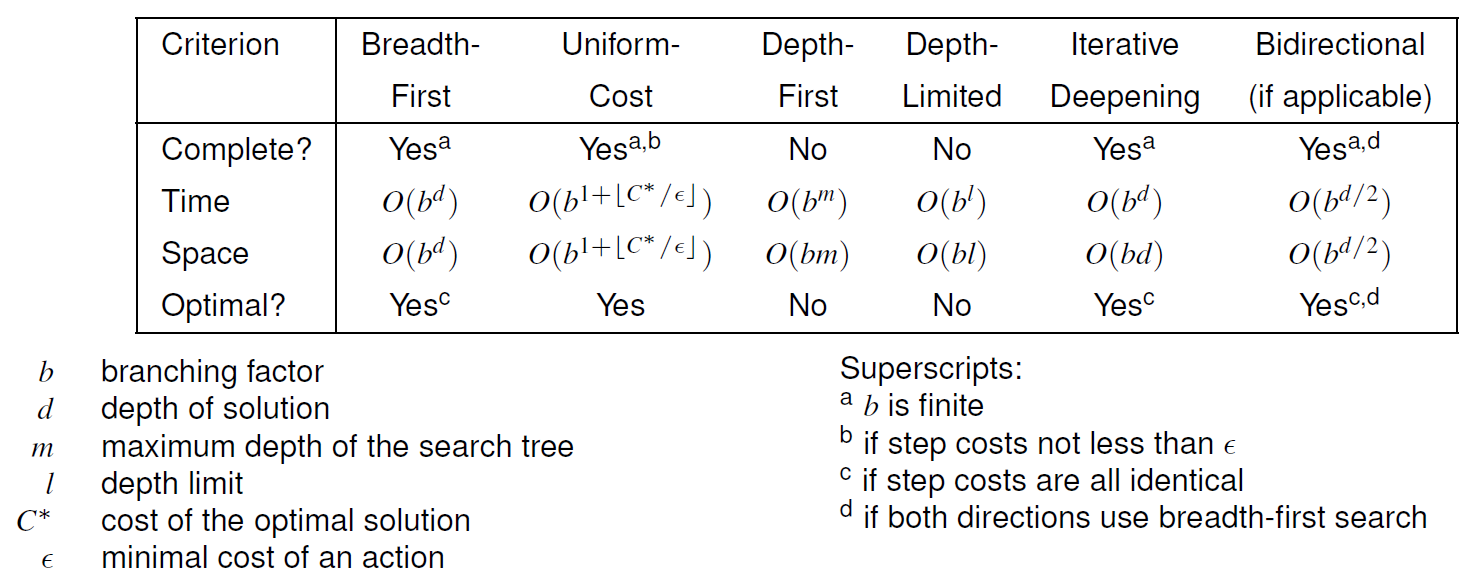
\includegraphics[width=0.7\textwidth]{searches.png}
\end{figure}